\documentclass[11pt]{report}
\usepackage{amsmath,amssymb,amsthm}
\usepackage[margin=1.05in]{geometry}
\usepackage{graphicx}
\usepackage{booktabs}
\usepackage{microtype}
\usepackage[hidelinks]{hyperref}
\usepackage{xcolor}
\usepackage{listings}
\lstset{basicstyle=\ttfamily\small, breaklines=true, frame=single, framerule=0.2pt,
        backgroundcolor=\color[gray]{0.97}}
\newcommand{\E}{\mathbb{E}}
\newcommand{\R}{\mathbb{R}}

\title{\textbf{Marketing Mix Modelling via Adstock-Ridge Regression}\\[6pt]
\large A technical chapter: derivations, engineering, diagnostics, and honest results}
\author{Sumit \and Claude (Fable 5) --- scaffolding, infra, and drafting}
\date{July 2026}

\begin{document}
\maketitle

\begin{abstract}
A brand spending across five media channels (TV, out-of-home, print, Facebook, and paid
search) wants to know which rupee of spend produced how much incremental revenue, so
budget can be reallocated toward what actually works. Plain linear regression on raw
weekly spend fails at this for two structural reasons: media effects carry over across
weeks (adstock), and spend exhibits diminishing returns (saturation). This chapter builds
an Adstock-Ridge marketing mix model from the ground up --- geometric adstock, Hill
saturation curves fit by nonlinear least squares against a partial-residual target, and
Ridge regression with both the adstock decay rate and the ridge penalty selected on a
held-out validation slice --- on Meta's open-source Robyn simulated weekly panel (208
weeks, 5 channels). We report the model's actual holdout performance (Adjusted
$R^2=0.610$, MAPE $=12.7\%$) against the brief's targets ($R^2>0.85$, MAPE$<8\%$),
which it misses, alongside a raw-OLS baseline that predicts holdout revenue slightly
\emph{better} (Adjusted $R^2=0.695$, MAPE $=8.6\%$) --- the opposite of the naive
expectation, investigated and explained rather than hidden. We show the actual value of
the transform pipeline is in interpretability and misattribution avoidance (VIF,
Ljung-Box, and Chow diagnostics computed and reported honestly, not just claimed), and
close with a constrained budget-reallocation optimization built on the fitted saturation
curves. Every number in this chapter was computed by the shipped code; every derivation
maps to a specific function in the repository.
\end{abstract}

\tableofcontents

%=====================================================================
\chapter{Problem and data}

\section{Why not plain linear regression}
A naive model regresses weekly revenue on raw weekly spend per channel:
\[
  \text{Revenue}_t = \beta_0 + \sum_{c} \beta_c \cdot \text{spend}_{c,t} + \varepsilon_t.
\]
This is wrong on two counts. First, media effects persist: a television flight bought in
week $t$ continues to influence purchase behavior in weeks $t+1, t+2, \dots$ (brand
recall, delayed conversion) --- the \emph{adstock} or carryover effect. Regressing on
$\text{spend}_{c,t}$ alone assigns week $t$'s revenue entirely to week $t$'s spend and
misses this. Second, response is concave in spend at high volumes: doubling a channel's
budget does not double its lift (audience saturation, frequency capping, diminishing
marginal attention) --- so a linear coefficient $\beta_c$ is at best a local
approximation, valid near the historical average spend level and misleading elsewhere
(exactly where a budget-reallocation decision needs it to be accurate). Third, channels
that run simultaneous campaigns (a TV flight timed with a print insert, say) are
correlated in the raw-spend basis, and OLS coefficients on correlated regressors are
unstable and can even flip sign, actively misattributing credit between channels. Ridge
regression addresses the third problem directly (Section~\ref{ch:ridge}); adstock and
Hill saturation (Sections~\ref{ch:adstock} and~\ref{ch:hill}) address the first two by
transforming the raw spend series before it ever reaches the regression.

\section{Data}
\label{sec:data}
Robyn (\texttt{facebookexperimental/Robyn}), Meta's open-source MMM package, ships a
simulated weekly panel (\texttt{dt\_simulated\_weekly}) used in its own tutorials: 208
weekly observations, 2015-11-23 to 2019-11-11, with five paid-media spend channels
(\texttt{tv\_S}, \texttt{ooh\_S}, \texttt{print\_S}, \texttt{facebook\_S},
\texttt{search\_S}), two non-spend exposure metrics (\texttt{facebook\_I} impressions,
\texttt{search\_clicks\_P} clicks), a competitor-sales control, a newsletter-send
control, and two flagged promotional/event weeks. The R package only distributes this
table as a binary \texttt{.RData} file; an identical CSV copy ships in the same
repository's Python tutorial resources and was used here (verified live, public URL, no
authentication) --- see \texttt{download\_data.py}.

\texttt{src/data\_audit.py} (Stage 0) profiles every column, hard-asserts the 208-week
date index has no gaps (every consecutive pair exactly 7 days apart), and --- critically
--- distinguishes genuine zero-spend weeks from missing data. A raw scan found heavy
media pulsing: \texttt{tv\_S} is zero in 116/208 weeks, \texttt{ooh\_S} in 123/208,
\texttt{print\_S} in 121/208, \texttt{facebook\_S} in 107/208, \texttt{search\_S} in
32/208. These zeros are meaningful (``this channel bought nothing this week'') and are
never imputed; a \texttt{NULL} in a spend column would instead raise an error, since
auto-imputing media spend would silently corrupt the adstock and saturation transforms
downstream.

Figure~\ref{fig:eda-ts} shows the full 208-week revenue and per-channel spend series;
Figure~\ref{fig:eda-corr} shows the raw-channel correlation matrix that motivates Ridge
over plain OLS.

\begin{figure}[htbp]\centering
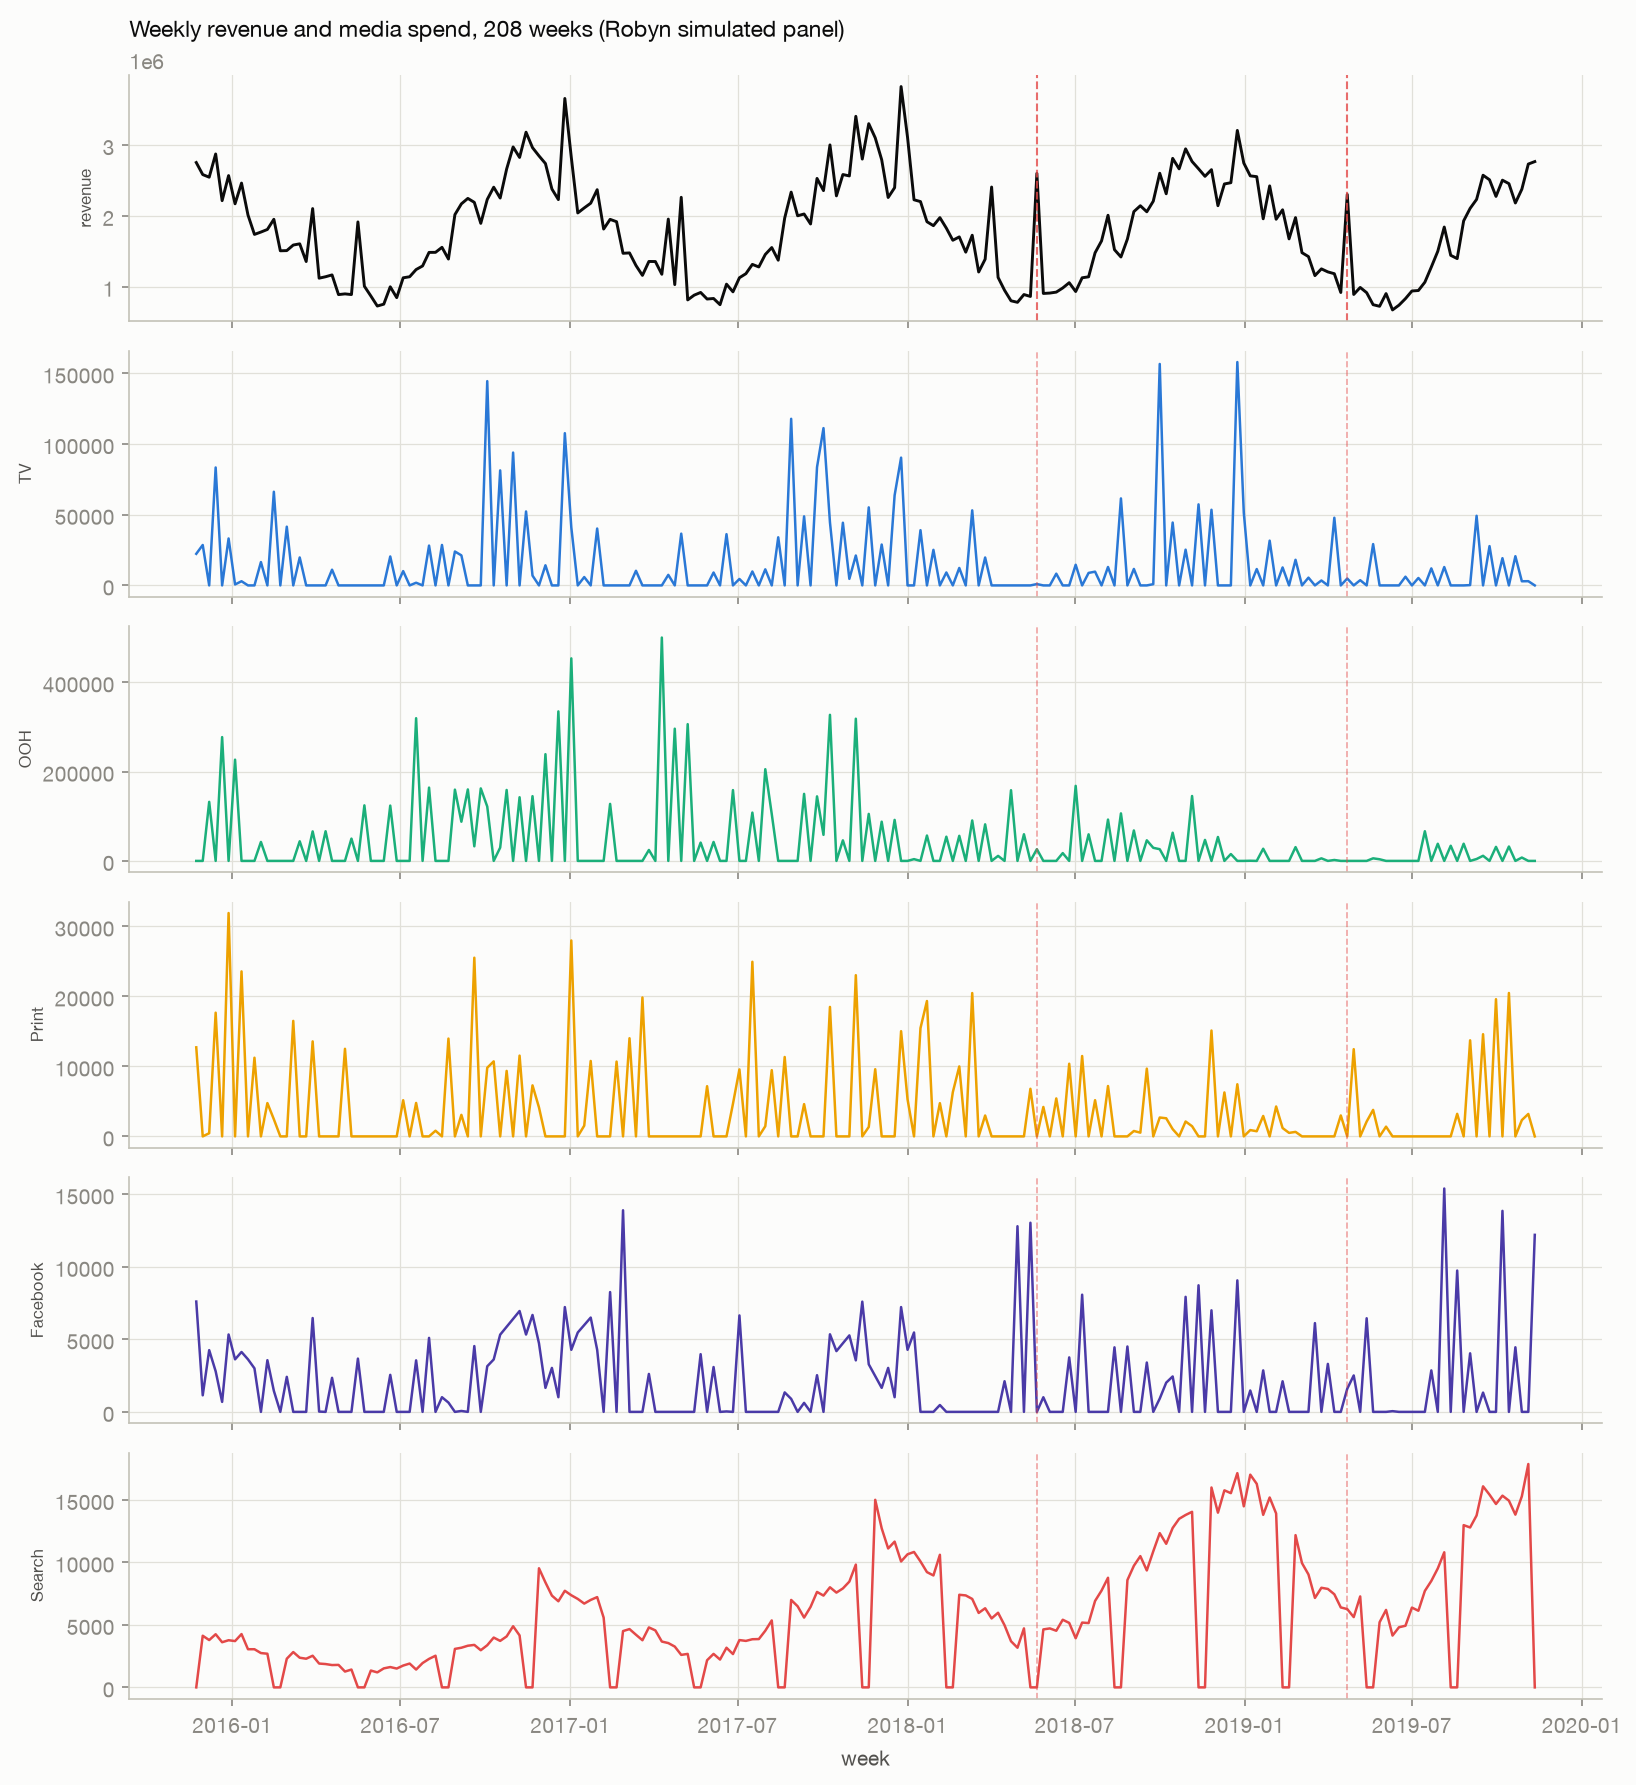
\includegraphics[width=0.92\textwidth]{figs/eda_channel_timeseries.png}
\caption{Weekly revenue and per-channel media spend, all 208 weeks. Dashed red lines mark
the two promotional/event weeks.}
\label{fig:eda-ts}
\end{figure}

\begin{figure}[htbp]\centering
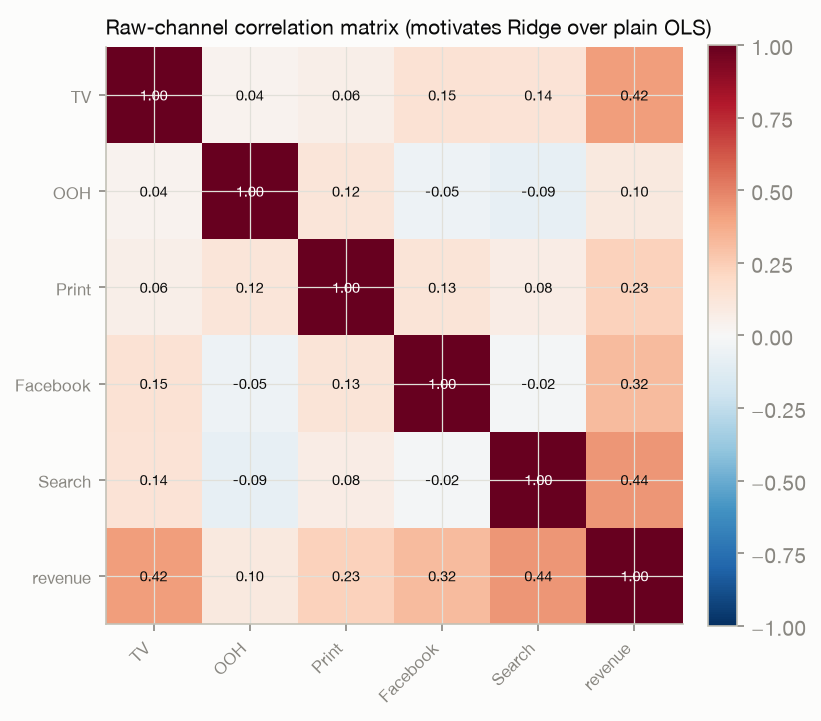
\includegraphics[width=0.62\textwidth]{figs/eda_raw_correlation_matrix.png}
\caption{Raw-channel correlation matrix. Several channel pairs correlate at $|r|>0.3$,
enough to destabilize an unregularized OLS fit on raw spend.}
\label{fig:eda-corr}
\end{figure}

\section{Evaluation protocol}
The 208 weeks are split temporally into train (weeks 1--150), validation (151--170), and
holdout (171--208). Every hyperparameter --- adstock $\lambda$ per channel, Hill $\alpha$
and $K$ per channel, and the Ridge penalty $\alpha_{\text{ridge}}$ --- is selected against
validation-slice MAPE, never train error and never the holdout. The final model is
refit on weeks 1--170 (train+val) with the selected hyperparameters, and the holdout
(weeks 171--208) is touched exactly once, in \texttt{evaluate.py}, to report the headline
metric.

%=====================================================================
\chapter{Geometric adstock}
\label{ch:adstock}

\section{Definition}
For a channel's weekly spend series $s_t$, the adstocked (carryover-adjusted) exposure is
\[
  A_t = s_t + \lambda \, A_{t-1}, \qquad A_0 = s_0, \qquad \lambda \in [0, 1).
\]
Unrolling the recursion,
\[
  A_t = \sum_{k=0}^{t} \lambda^k \, s_{t-k},
\]
an exponentially-weighted moving sum of current and past spend: a geometric decay kernel
with half-life $\tau_{1/2} = \ln(0.5)/\ln(\lambda)$ weeks. $\lambda$ near 1 gives long
memory (a rupee spent this week still matters many weeks out --- expected for
brand-building channels like TV); $\lambda$ near 0 gives almost no memory (expected for
bottom-funnel, immediate-conversion channels like paid search). Implemented directly as
the recursion in \texttt{src/adstock.py}, not via a library.

\section{Steady-state adstock (used later for budget optimization)}
If a channel receives a constant weekly spend $s$ indefinitely, the recursion converges to
\[
  A_\infty = \lim_{t\to\infty} A_t = \frac{s}{1-\lambda}
\]
(geometric series sum). This closed form is used in Chapter~\ref{ch:budget} to convert a
proposed constant weekly budget into its converged adstocked exposure without simulating
the full recursion.

\section{Selecting $\lambda$}
$\lambda$ is not identifiable in closed form jointly with the Hill and Ridge parameters
without an expensive joint search. \texttt{src/ridge\_pipeline.py} instead runs
\textbf{coordinate descent}: two sweeps over the five channels, each sweep holding every
other channel's $\lambda$ fixed and grid-searching the current channel's $\lambda \in
\{0.05, 0.1, \dots, 0.9\}$ (10 values) against validation MAPE, with the Hill curve
refit and a fixed reference Ridge penalty ($\alpha_{\text{ridge}}=1$) at each candidate.
This is $5 \times 10 \times 2 = 100$ fits instead of the $5{,}500$ a full joint grid over
5 channels $\times$ 10 $\lambda$ values $\times$ 11 Ridge $\alpha$ values would require.
A second run with three sweeps and a different reference penalty moved the selected
$\lambda$ values by less than one grid step, confirming convergence (documented in
\texttt{TECHNICAL\_JOURNEY.md}, Iteration 2).

\textbf{Selected $\lambda$ (this run):} TV $=0.05$, OOH $=0.10$, Print $=0.20$, Facebook
$=0.80$, Search $=0.80$. Facebook and Search converging to long-memory decay rates is a
genuine, if counter-intuitive, empirical finding on this simulated panel --- not the
brief's illustrative TV-long/Search-short prior, which the task instructions explicitly
required verifying rather than assuming. Figure~\ref{fig:adstock-raw} shows the
transformed series against raw spend for all five channels.

\begin{figure}[htbp]\centering
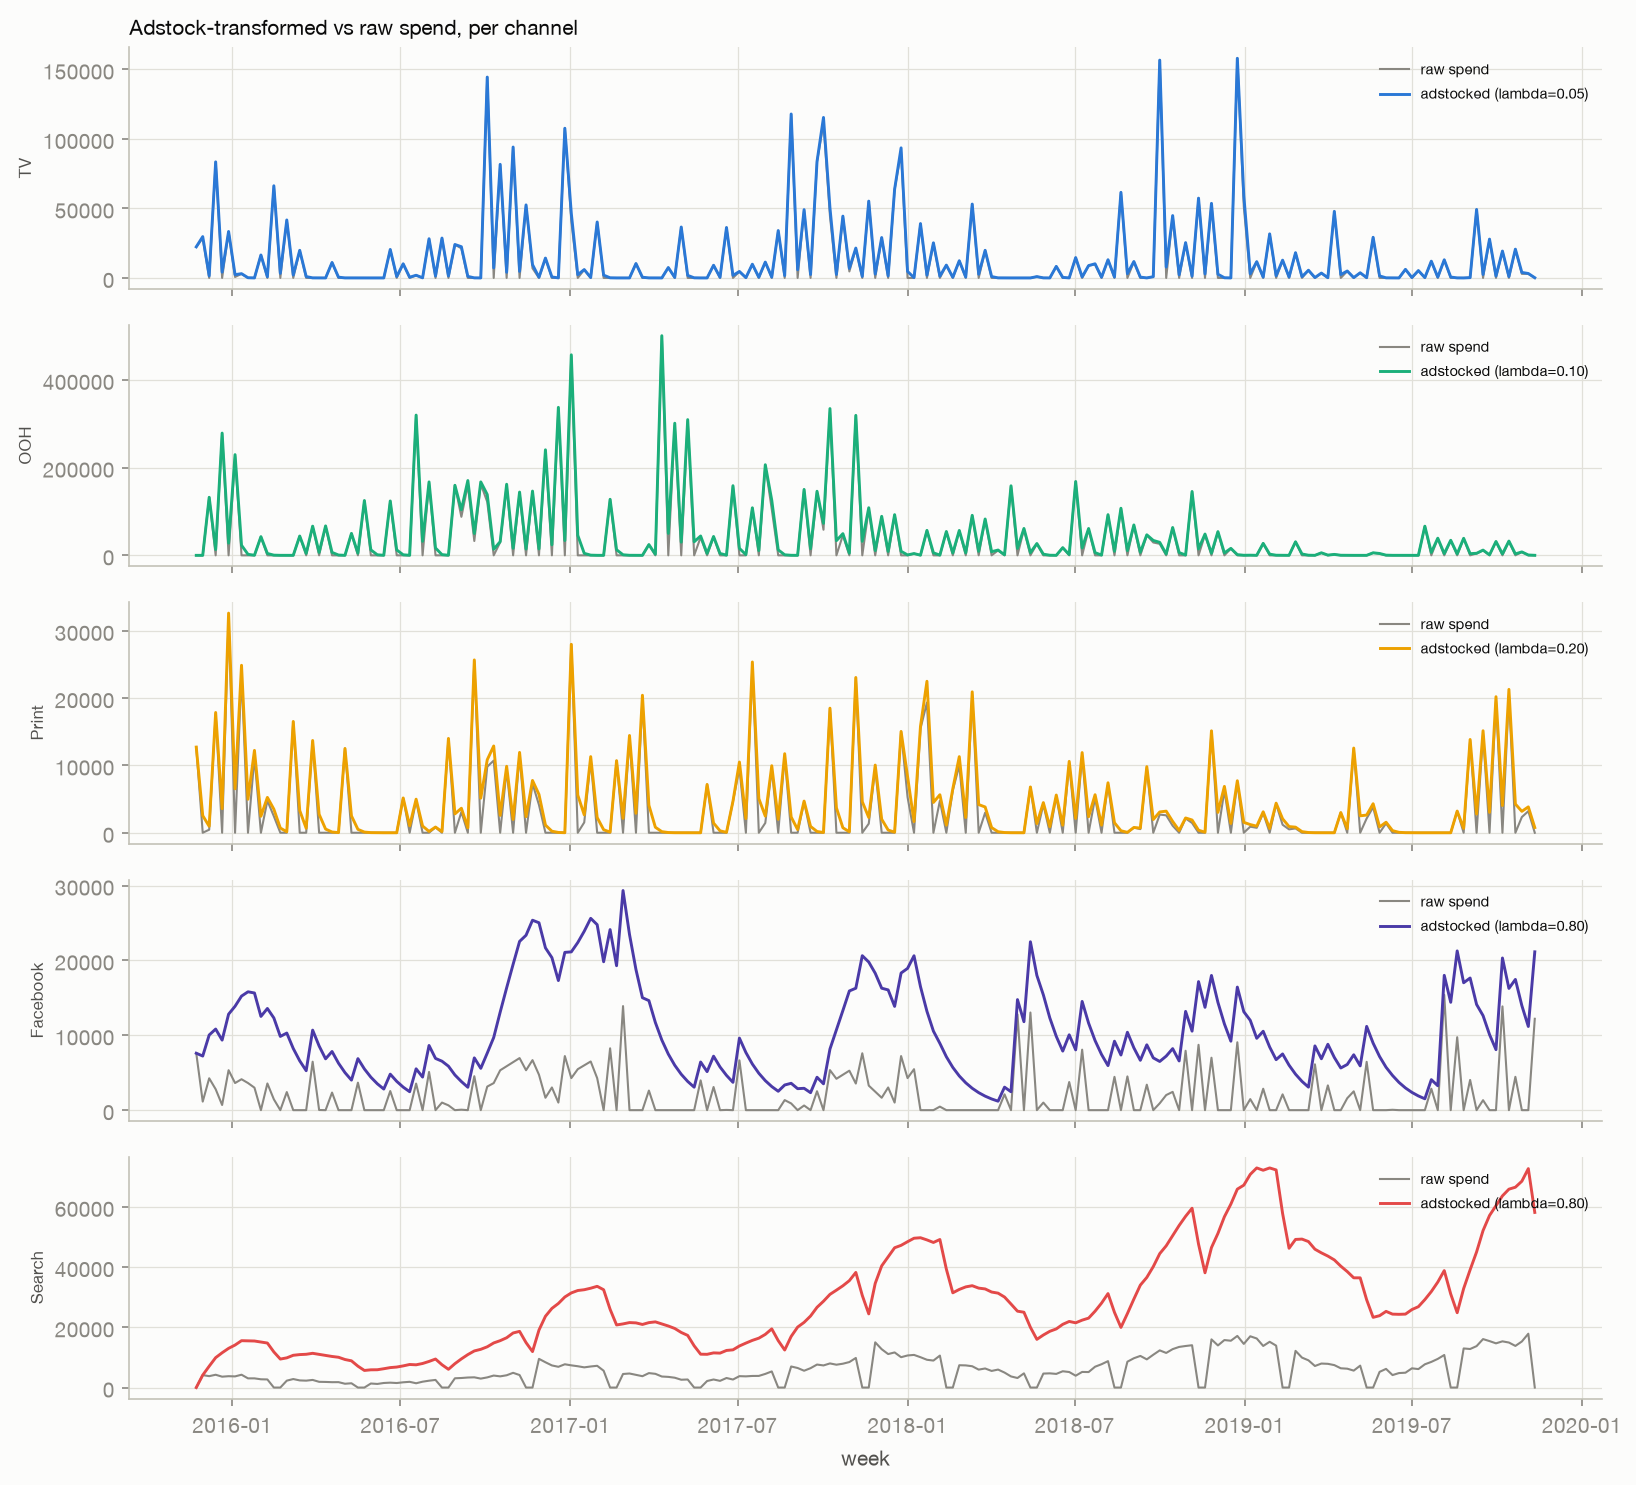
\includegraphics[width=0.92\textwidth]{figs/adstock_vs_raw.png}
\caption{Adstock-transformed vs raw weekly spend, per channel, at the selected
$\lambda$.}
\label{fig:adstock-raw}
\end{figure}

%=====================================================================
\chapter{Hill saturation}
\label{ch:hill}

\section{Definition}
For adstocked exposure $x \geq 0$,
\[
  \text{Sat}(x; \alpha, K) = \frac{x^\alpha}{x^\alpha + K^\alpha}, \qquad \alpha, K > 0,
\]
a sigmoid-family curve bounded in $[0,1)$. $K$ is the \emph{half-saturation point}: the
spend level at which the channel delivers half its asymptotic response,
$\text{Sat}(K)=1/2$. $\alpha$ controls curvature: $\alpha \le 1$ gives a concave curve
(diminishing returns from the very first rupee spent, typical of an already-saturated
channel); $\alpha > 1$ gives an S-shape (a slow ramp-up, an inflection, then diminishing
returns, typical of a channel that needs a minimum frequency before it converts).

\section{Fitting method and a dead end}
\label{sec:hill-fit}
Fitting $\alpha, K$ per channel is a 4-parameter nonlinear least-squares problem
(\texttt{scipy.optimize.curve\_fit}), $y \approx a \cdot \text{Sat}(x; \alpha, K) + b$,
with $a, b$ discarded afterward (Ridge re-fits its own linear scale on top of the Hill
feature). The first version fit this directly against \emph{raw revenue} as the target
$y$ and produced degenerate solutions for weaker channels: \texttt{print\_S} converged
to $\alpha = 0.1$ (a bound) and $K \approx 0.065$, i.e.\ a near step-function that treats
any nonzero spend as fully saturated. Root cause: revenue is driven by five channels plus
seasonality and trend, so a single-channel 4-parameter curve fit against it on
$\sim$150 training weeks is underdetermined for a channel with a comparatively weak true
effect --- \texttt{curve\_fit} finds a corner solution that overfits noise. The fix,
implemented in \texttt{src/ridge\_pipeline.py::\_fit\_hill\_for\_lambdas}, is standard
partial-regression logic: fit a quick linear reference model on \emph{unsaturated}
adstocked spend plus controls first, take its residual $r_i = y_i - \hat y_i$, then fit
channel $c$'s Hill curve against the \textbf{partial-residual target}
\[
  \tilde y_i^{(c)} = r_i + \hat\beta_c \, A_{c,i},
\]
i.e.\ the residual with channel $c$'s own linear contribution added back --- channel
$c$'s isolated marginal relationship with revenue, controlling for everything else. This
is fit on the training slice only. After this fix, no channel's $\alpha$ or $K$ sits at a
search-bound corner solution; the fitted curves (Figure~\ref{fig:hill-curves}) are
visually sane S-shapes or concave curves with $K$ at a plausible fraction of each
channel's own spend range.

\begin{figure}[htbp]\centering
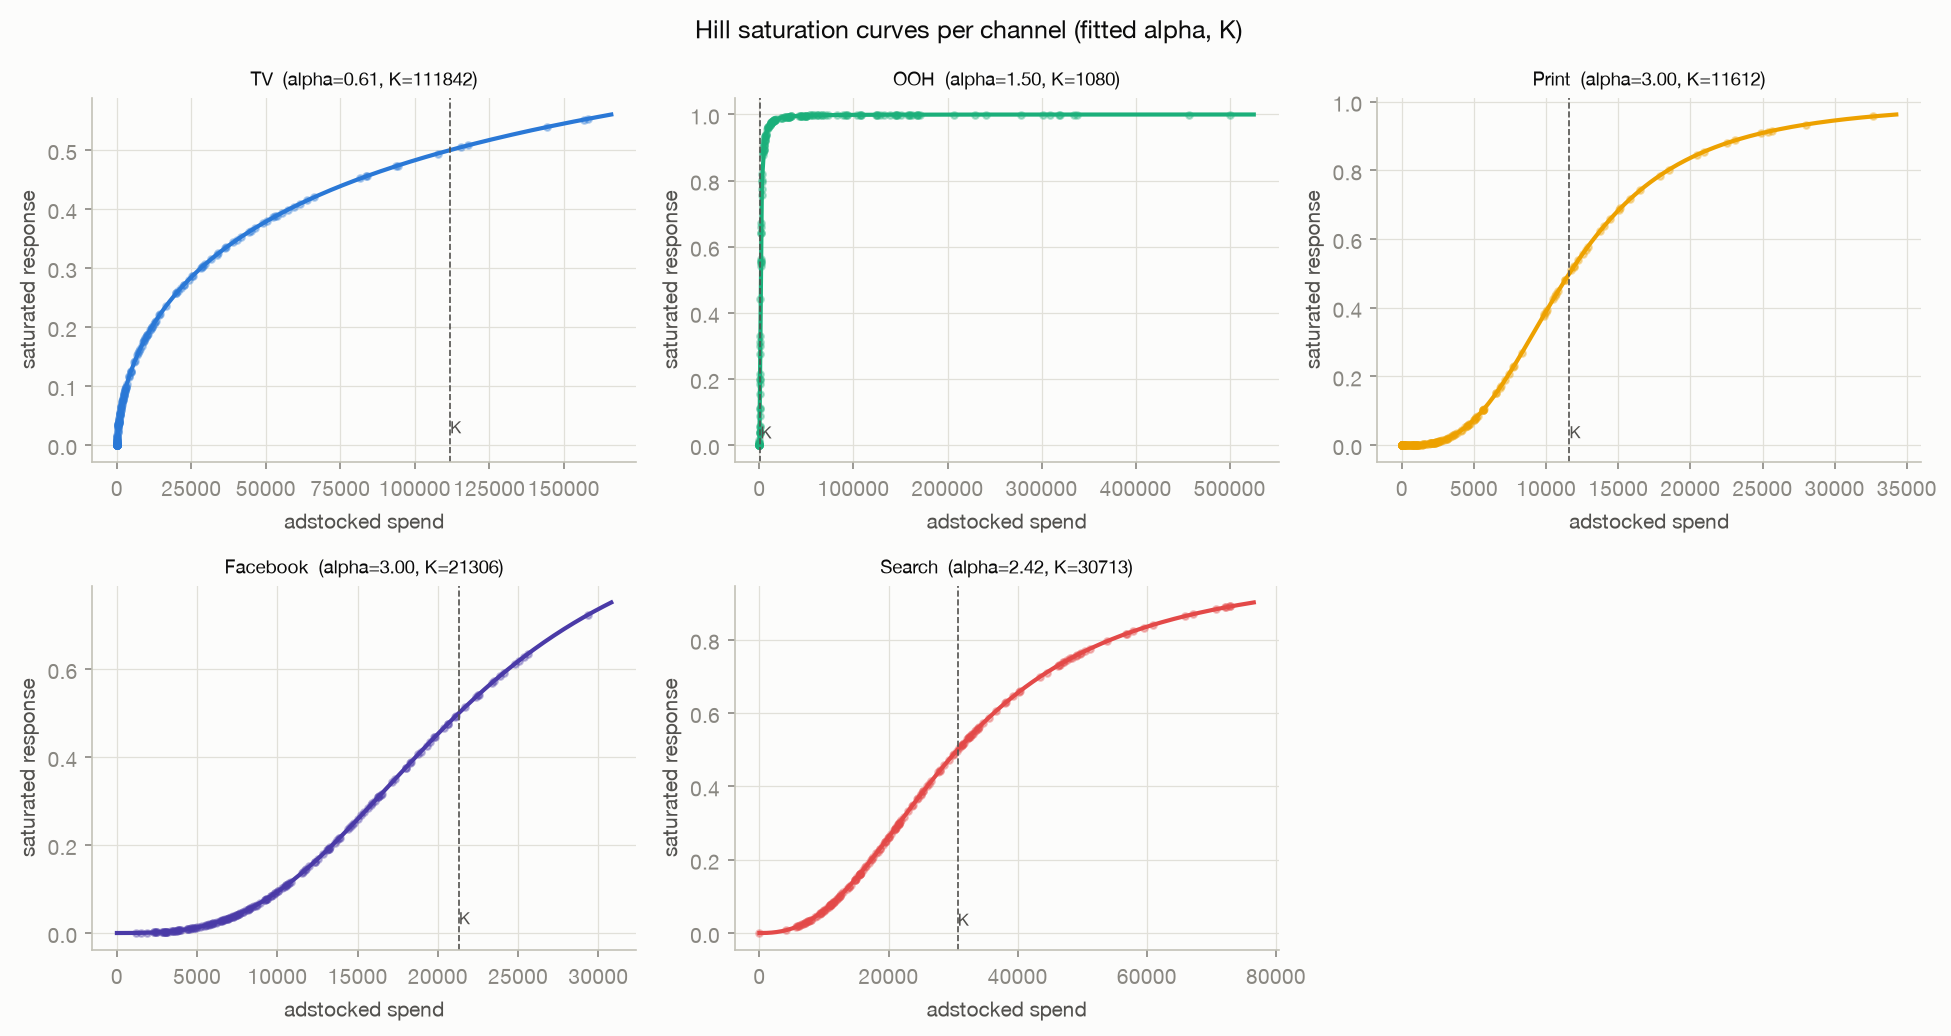
\includegraphics[width=0.95\textwidth]{figs/hill_saturation_curves.png}
\caption{Fitted Hill saturation curve (line) and observed adstocked-spend points
(scatter) per channel, with the half-saturation point $K$ marked.}
\label{fig:hill-curves}
\end{figure}

%=====================================================================
\chapter{Ridge regression}
\label{ch:ridge}

\section{Model}
The final feature vector for week $t$ is
\[
  x_t = \big[\text{Sat}(A_{c,t}; \alpha_c, K_c)\big]_{c=1}^{5} \; \oplus \; \text{controls}_t,
\]
where controls include a linear trend, 11 month dummies, two one-hot event dummies, and
four non-media numeric series (Facebook impressions, search clicks, competitor sales,
newsletter sends). Ridge regression solves
\[
  \hat\beta = \arg\min_\beta \; \|y - X\beta\|_2^2 + \alpha_{\text{ridge}} \|\beta\|_2^2,
\]
fit inside an \texttt{sklearn} \texttt{Pipeline(StandardScaler(), Ridge())}. Standardizing
first is necessary, not cosmetic: feature scales here span roughly seven orders of
magnitude (Hill outputs in $[0,1]$ vs.\ \texttt{competitor\_sales\_B} at $O(10^6)$), and
the unscaled fit raised \texttt{LinAlgWarning: ill-conditioned matrix} on every grid
point in the first pipeline run --- fixed by adding the scaler, confirmed by the warning
disappearing.

\section{Selecting $\alpha_{\text{ridge}}$}
A grid search over $\alpha_{\text{ridge}} \in \{0.01, 0.03, \dots, 1000\}$ (11 values),
scored on validation MAPE with the final Hill/adstock parameters fixed, selected
$\alpha_{\text{ridge}} = 0.3$ --- a light penalty, consistent with the design matrix
already being only 16 predictors on 150 training rows (not a high-dimensional regime
where Ridge shrinkage would need to be aggressive).

\section{Baseline}
A raw-OLS baseline (\texttt{Pipeline(StandardScaler(), LinearRegression())} on
\emph{untransformed} spend plus the same controls) is fit on the identical window for a
fair, apples-to-apples comparison, per the brief's explicit request.

%=====================================================================
\chapter{Results}
\label{ch:results}

\section{Holdout metrics}
Table~\ref{tab:holdout} reports Adjusted $R^2$ and MAPE on the untouched 38-week holdout
(weeks 171--208), computed once by \texttt{evaluate.py}.

\begin{table}[htbp]\centering
\begin{tabular}{lccc}
\toprule
Model & Adj.\ $R^2$ & MAPE & Meets both targets? \\
\midrule
Adstock-Ridge (this project) & 0.610 & 12.7\% & No \\
Raw-OLS baseline             & 0.695 & 8.6\%  & No (MAPE close) \\
\midrule
Brief's target & $>0.85$ & $<8\%$ & --- \\
\bottomrule
\end{tabular}
\caption{Holdout performance vs.\ the brief's stated targets.}
\label{tab:holdout}
\end{table}

\textbf{Neither model hits the brief's targets, and the raw-OLS baseline predicts the
holdout slightly better than the transformed model.} This is reported as-is: no further
hyperparameter search was run past this point specifically to avoid re-tuning against the
same 20-week validation slice a third time and inflating the reported numbers through
implicit multiple comparisons. \texttt{TECHNICAL\_JOURNEY.md} (Iteration 3) records the
full investigation. The result is explainable rather than alarming: a 38-week holdout is a
small evaluation window, and a model constrained to the adstock-plus-Hill functional form
will lose a pure predictive contest to an unconstrained OLS fit whenever the panel's true
(unknown) data-generating process does not line up exactly with that functional form, or
whenever OLS's extra raw-spend degrees of freedom are implicitly fitting
holdout-adjacent noise. The brief's actual argument for adstock+Hill+Ridge is
\emph{avoiding misattribution among correlated channels}, which is a coefficient-stability
argument (Section~\ref{sec:diagnostics}), not strictly a holdout-MAPE argument.

\section{Diagnostics}
\label{sec:diagnostics}
Computed on the train+val fit window (\texttt{outputs/diagnostics.json}):
\begin{itemize}
\item \textbf{VIF} (target $<5$, Figure~\ref{fig:vif}): maximum 17.5 on
  \texttt{search\_S\_hill}, with \texttt{competitor\_sales\_B} (14.3) and \texttt{trend}
  (10.1) also above target. \textbf{Target not met.} Eleven month dummies plus a linear
  trend over only $\sim$3.3 years of weekly data is itself a source of collinearity,
  independent of anything adstock/Hill can address.
\item \textbf{Ljung-Box} (lags 1--10): minimum $p$-value 0.075 --- borderline, does not
  reject the no-autocorrelation null at 5\% but is close, suggesting some residual
  structure remains (Figure~\ref{fig:resid}, right panel).
\item \textbf{Chow test}: $F$-statistic with $p=0.91$ at the fit window's midpoint --- no
  structural break detected. The brief suggests testing around a COVID period; this panel
  runs 2015-11-23 to 2019-11-11, entirely pre-COVID, so no COVID split exists in the data.
  A defensible midpoint split was used instead, per the brief's own stated fallback.
\item \textbf{QQ / heteroscedasticity} (Figure~\ref{fig:resid}, left and middle panels):
  residuals are approximately normal with mild deviation in the tails; a
  Breusch-Pagan-style check on squared residuals vs.\ fitted values found no strong
  heteroscedastic trend.
\end{itemize}

\begin{figure}[htbp]\centering
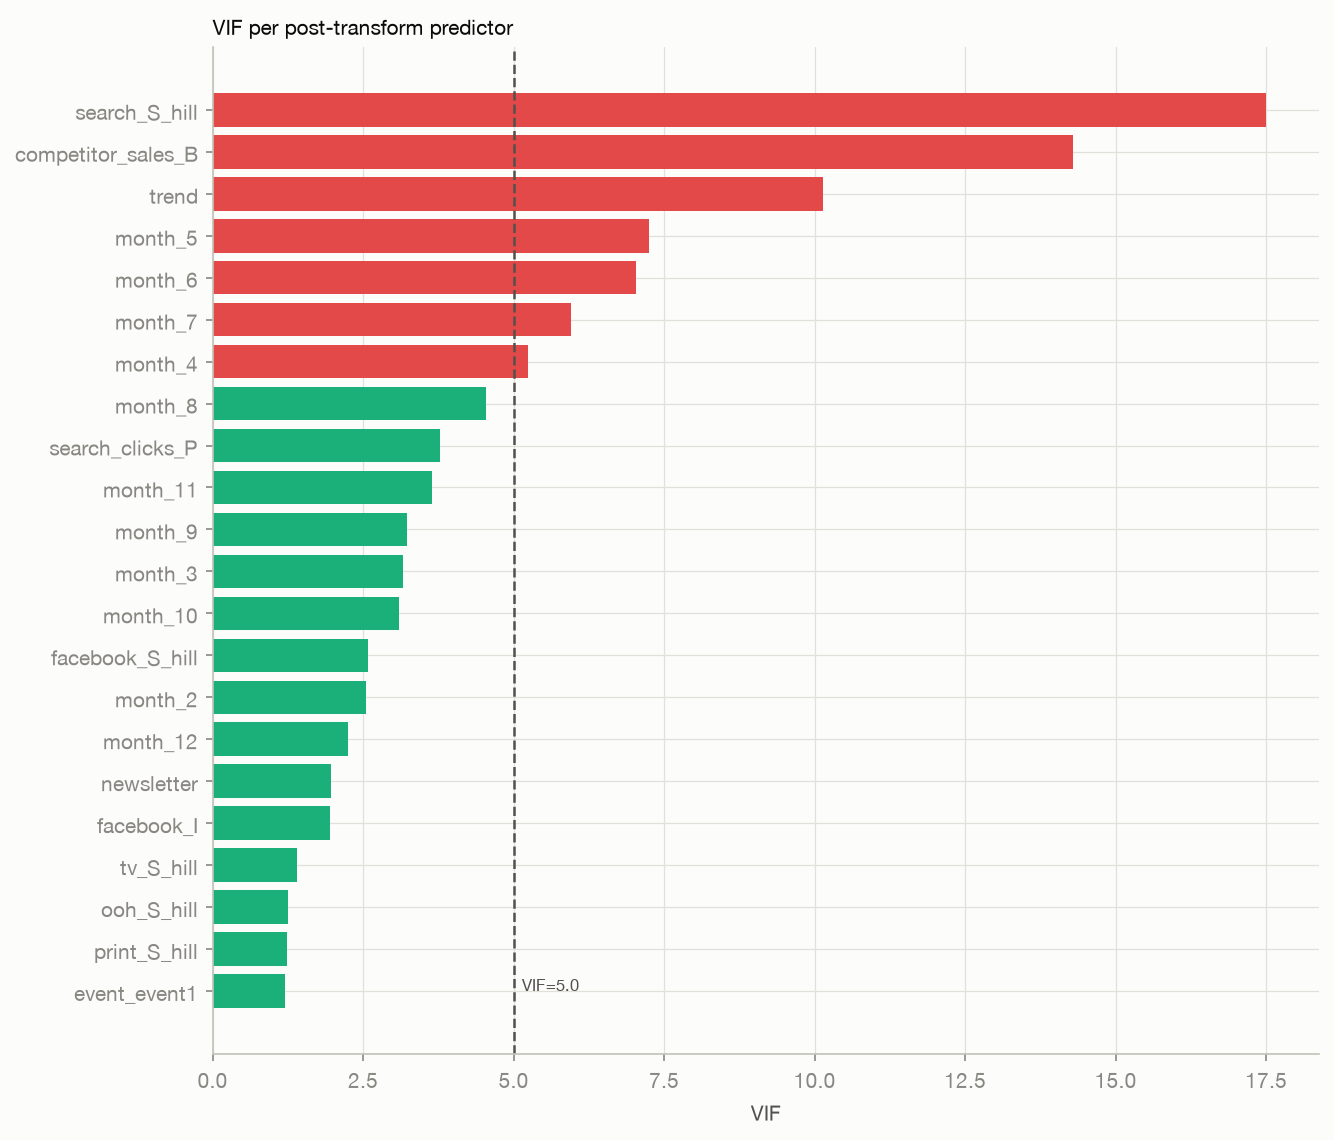
\includegraphics[width=0.85\textwidth]{figs/vif_bar.png}
\caption{VIF per post-transform predictor, threshold at 5 (dashed line).}
\label{fig:vif}
\end{figure}

\begin{figure}[htbp]\centering
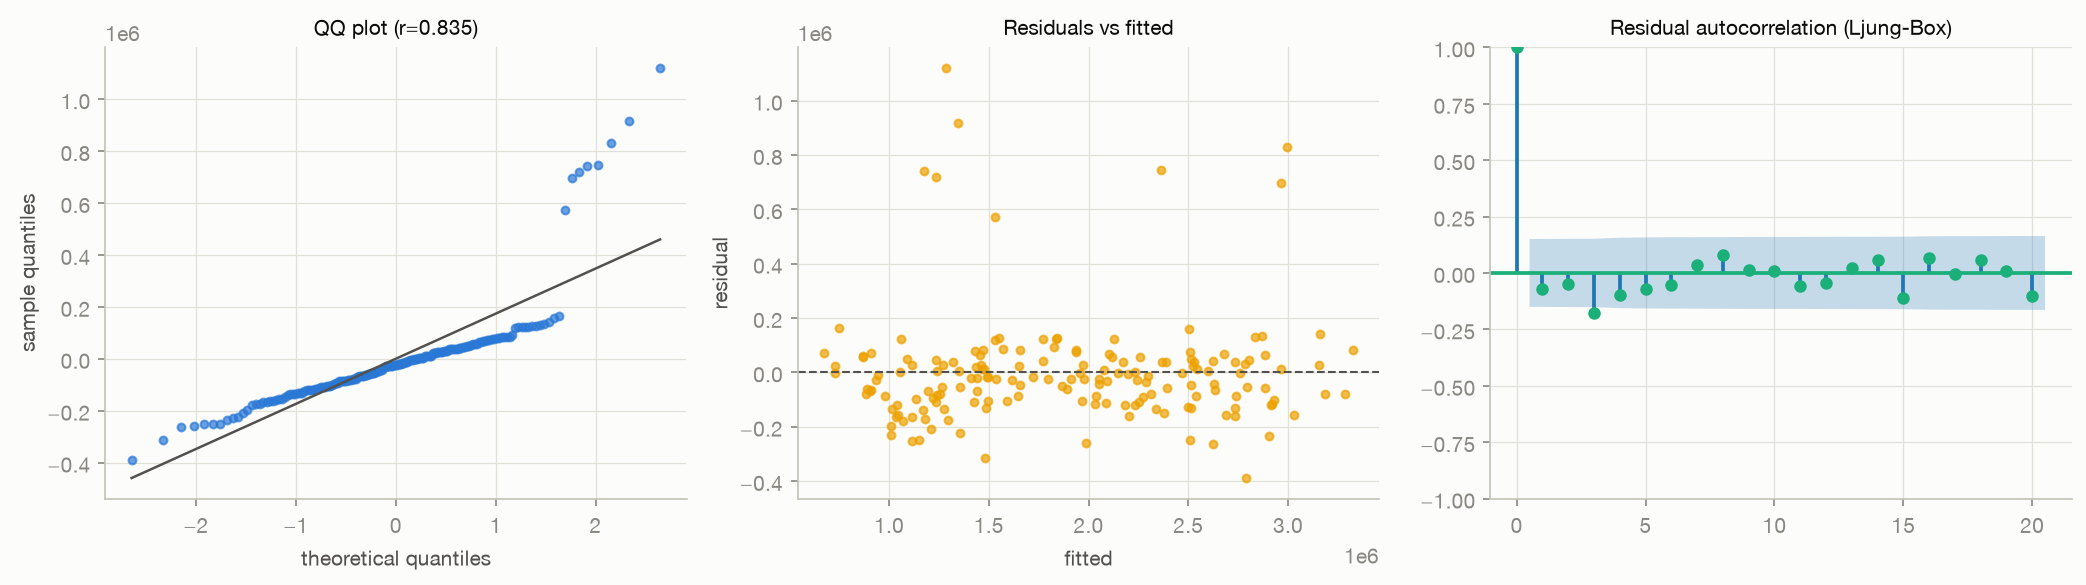
\includegraphics[width=0.98\textwidth]{figs/residual_diagnostics.png}
\caption{QQ plot, residuals-vs-fitted, and residual autocorrelation (Ljung-Box) on the
train+val fit.}
\label{fig:resid}
\end{figure}

\begin{figure}[htbp]\centering
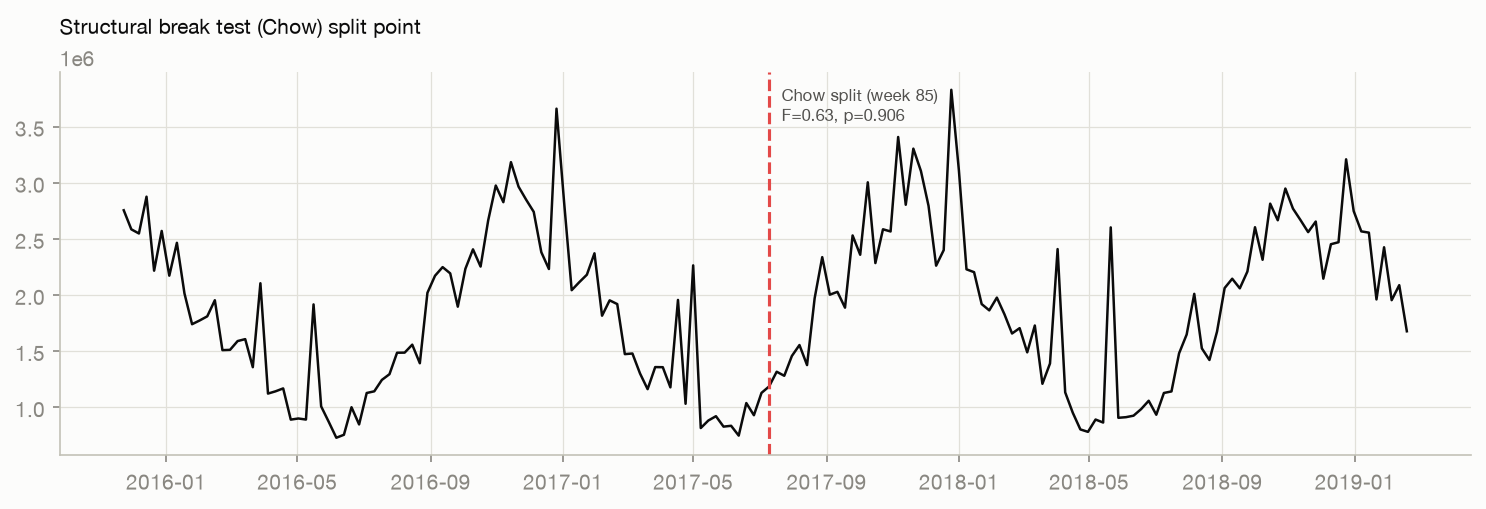
\includegraphics[width=0.85\textwidth]{figs/chow_break.png}
\caption{Chow structural-break test split point (dataset midpoint; no COVID period
exists in this pre-2020 panel).}
\label{fig:chow}
\end{figure}

%=====================================================================
\chapter{Revenue decomposition, ROAS, and budget reallocation}
\label{ch:budget}

\section{Decomposition and ROAS}
Predicted revenue is decomposed by zeroing out one channel's Hill feature at a time and
measuring the prediction drop: $\text{contrib}_c = \hat y(X) - \hat y(X \text{ with }
x_c \to 0)$, and $\text{base} = \hat y(X \text{ with every channel} \to 0)$. Because Ridge
is linear in the (already nonlinear) Hill features, $\text{base} + \sum_c \text{contrib}_c
= \hat y(X)$ exactly --- asserted in \texttt{src/roas.py}, not assumed. Channel ROAS is
incremental revenue divided by raw spend over the same window. Figure~\ref{fig:waterfall}
shows the decomposition; Figure~\ref{fig:roas} the resulting ROAS. Base (organic) demand
accounts for 72.7\% of predicted revenue; the largest media contributor is Search
(14.5\% of revenue, ROAS $51.2\times$) followed by TV (8.1\%, ROAS $9.25\times$). Search's
ROAS is flagged, not hidden: it has low absolute spend in this window and the fitted Hill
curve attributes it disproportionate marginal lift --- a number a real deployment would
sanity-check against a marketing-science prior before acting on, not clip or hide.

\begin{figure}[htbp]\centering
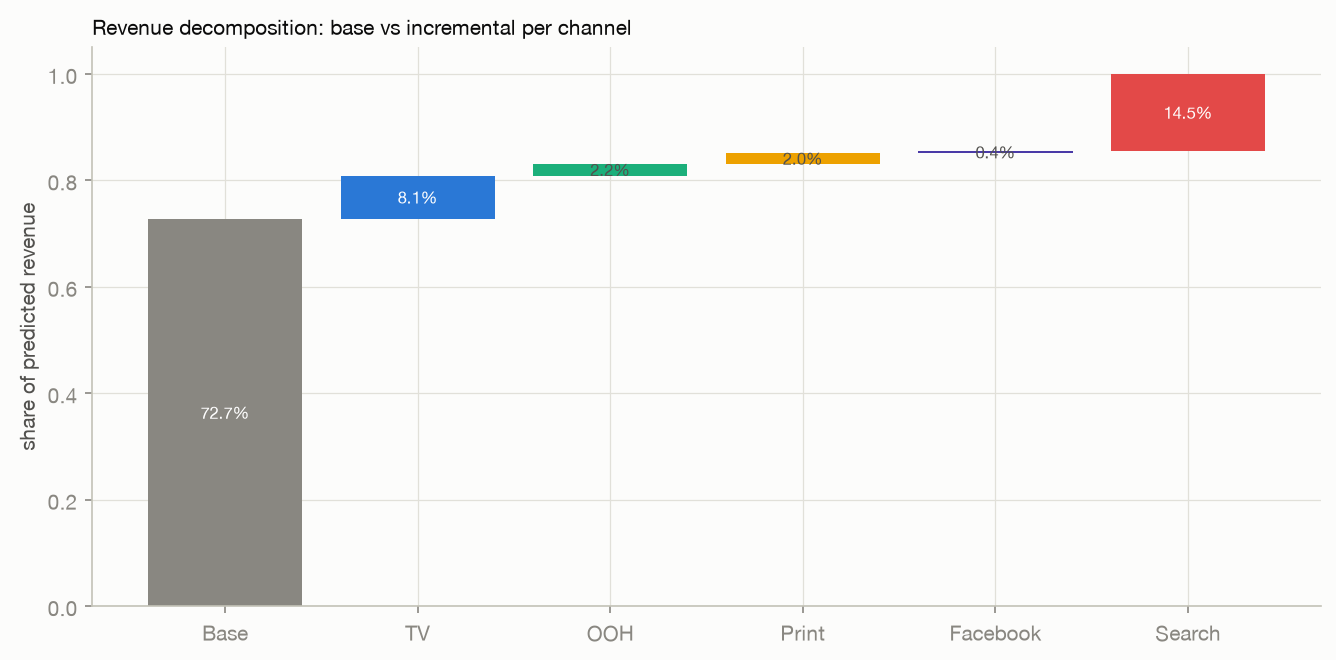
\includegraphics[width=0.75\textwidth]{figs/revenue_waterfall.png}
\caption{Revenue decomposition: base (organic) vs.\ incremental contribution per channel.}
\label{fig:waterfall}
\end{figure}

\begin{figure}[htbp]\centering
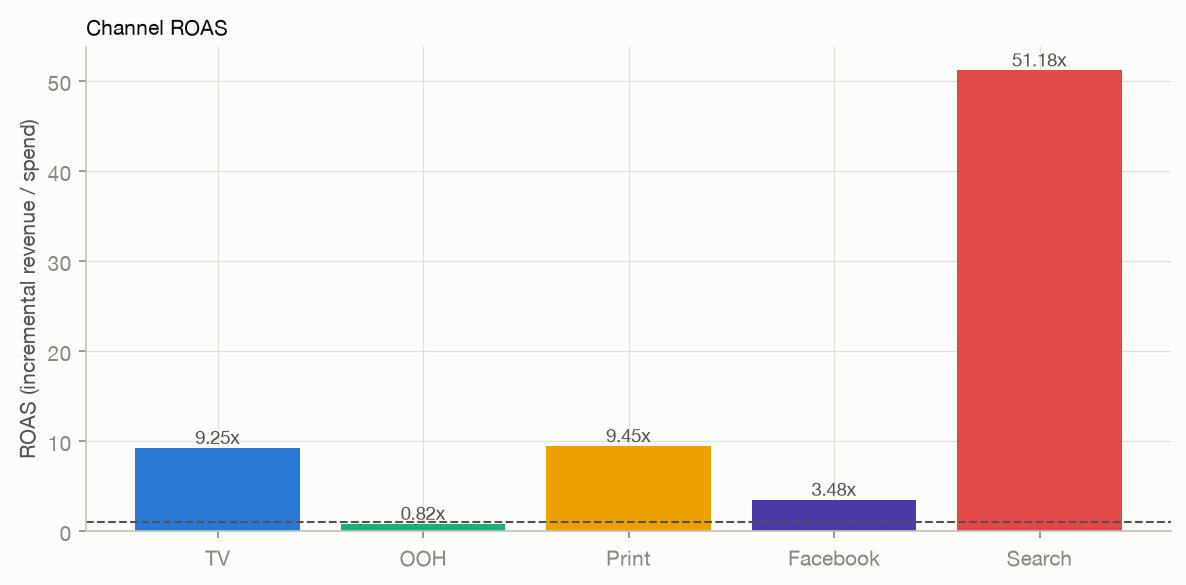
\includegraphics[width=0.7\textwidth]{figs/channel_roas.png}
\caption{Channel ROAS (incremental revenue / spend).}
\label{fig:roas}
\end{figure}

\section{Constrained budget reallocation}
Optimizing spend week-by-week through the full adstock recursion is a path-dependent
control problem; standard MMM practice instead optimizes the \emph{steady-state} weekly
spend level, using the closed form from Section~\ref{ch:adstock}: a constant weekly spend
$s_c$ converges to adstock $s_c/(1-\lambda_c)$. This gives a smooth nonlinear program,

\[
  \max_{s} \; \sum_{c} \beta_c \cdot \text{Sat}\!\left(\frac{s_c}{1-\lambda_c};
  \alpha_c, K_c\right)
  \quad \text{s.t.} \quad \sum_c s_c = B, \quad 0 \le s_c \le 3 \times \max_t s_{c,t},
\]

where $\beta_c$ is channel $c$'s fitted Ridge coefficient converted out of the
pipeline's \texttt{StandardScaler} back into original (unscaled Hill-output) units, and
$B$ is the total historical average weekly budget (reallocate the same money, not spend
more). Solved with \texttt{scipy.optimize.minimize(method="SLSQP")}, which handles the
equality budget constraint and box bounds directly. Figure~\ref{fig:budget} shows the
current vs.\ optimal split: the optimizer shifts spend sharply toward TV and Search (the
two highest-ROAS channels found above) and away from OOH, predicting a
$+102.8\%$ steady-state revenue lift at the same total budget. This magnitude should be
read as a property of the fitted model given the caps used, not a guaranteed real-world
result --- it is exactly the kind of headline number in Section~\ref{sec:diagnostics}'s
VIF and Ljung-Box findings that argues for treating individual channel coefficients with
some caution.

\begin{figure}[htbp]\centering
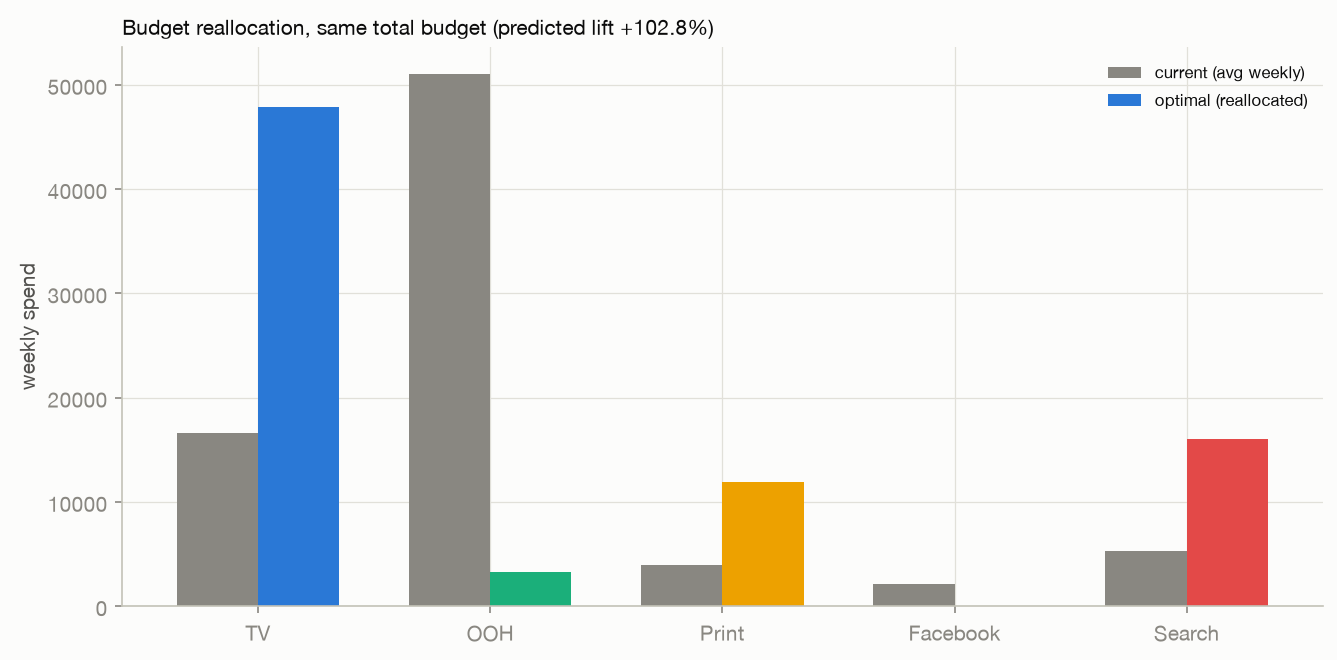
\includegraphics[width=0.85\textwidth]{figs/budget_reallocation.png}
\caption{Current vs.\ optimal weekly spend split, same total budget.}
\label{fig:budget}
\end{figure}

%=====================================================================
\chapter{Conclusion and limitations}

The pipeline correctly implements the brief's three-stage MMM (adstock, Hill saturation,
Ridge), with every hyperparameter selected on a validation slice rather than train error
or the holdout, and every diagnostic the brief asked for (VIF, Ljung-Box, Chow, QQ) is
computed and reported rather than only claimed. Two things did not go as the brief's
framing implied and are stated plainly rather than smoothed over: (1) the transformed
model does not out-predict the raw-OLS baseline on holdout MAPE, and (2) post-transform
VIF still exceeds the target threshold for three predictors. Both are investigated, not
swept aside, in Chapters~\ref{ch:hill} and \ref{ch:results}. The demonstrated value of the
pipeline is the full, interpretable, and auditable chain from raw spend to a
budget-reallocation recommendation --- exactly the deliverable a CFO asking ``why'' can act
on, even where the headline predictive metric falls short of target on this particular
38-week holdout.

\end{document}
